\documentclass[12pt]{article}
\usepackage{graphics,textcomp}
\newcommand{\micro}{\hbox{\textmu}}
\newcommand{\unit}[1]{\mathrm{#1}}
  \renewcommand{\deg}{\unit{deg}}
  \newcommand{\rad}{\unit{rad}}
  \newcommand{\s}{\unit{s}}
  \newcommand{\ns}{\unit{ns}}
  \newcommand{\m}{\unit{m}}
    \newcommand{\mps}{\m\,\s^{-1}}
  \newcommand{\cm}{\unit{cm}}
  \newcommand{\mm}{\unit{mm}}
  \newcommand{\mum}{\unit{\micro m}}
  \newcommand{\nm}{\unit{nm}}
  \newcommand{\Hz}{\unit{Hz}}
\newcounter{answer}
\newenvironment{alist}{\begin{list}{(\Alph{answer})}{\usecounter{answer}}}%
  {\end{list}}
\newcommand{\explicitcorrect}[1]{[({#1})~\textbf{correct}]}
\newcommand{\correct}{~[\textbf{correct}]}
\newcommand{\source}[1]{\textsl{#1}}
\renewcommand{\emph}[1]{\textbf{#1}}
\begin{document}
\raggedright
\begin{enumerate}

\item \source{(from lecture, 2009-01-21)} Which of the following
  expressions could \emph{not} be the wave speed in a string?
  \emph{Hint:} Think about the dimensions or units.\begin{alist}
    \item $\displaystyle\omega\,k\quad$, where $\omega$ is angular
      frequency and $k$ is wave number\correct
    \item $\displaystyle\frac{\lambda}{T}\quad$, where $\lambda$ is
      wavelength and $T$ is period
    \item $\displaystyle\sqrt{\frac{F\,L}{M}}\quad$, where $F$ is force,
      $L$ is length, and $M$ is mass
    \item $\displaystyle\sqrt{\frac{T}{\mu}}\quad$, where $T$ is tension,
      and $\mu$ is mass per unit length
  \end{alist}

\item \source{(from Chapter 21 homework)} A musical instrument is
  illustrated below. Six pieces of identical piano wire (cut to
  different lengths) are hung from the same support, and masses are
  hung from the free end of each wire. Each wire is 1, 2, or 3 units
  long, and each supports 1, 2, or 4 units of mass. The mass of each
  wire is negligible compared to the total mass hanging from it.
  Which of the strings A through E has the lowest fundamental
  frequency of standing-wave
  vibration?\\ \resizebox{2in}{!}{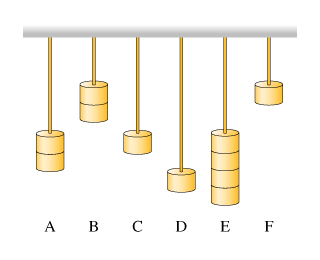
\includegraphics{1011705.jpg}}\\
  \explicitcorrect{D}

\item \source{(from conceptual question 21.2)} If you take snapshots of
  a standing wave on a string, there are certain instants when the
  string is at maximum displacement (maximum amplitude).  In what form
  is the energy in the wave at those instants?\begin{alist}
    \item kinetic energy
    \item potential energy\correct
    \item thermal energy
    \item a standing wave contains no energy
    \item there is no such thing as energy ``at an instant''
  \end{alist}

\item \source{(from lecture, 2009-01-26)} An organ pipe is long and thin
  and open at one end, closed at the other.  The fundamental frequency
  is $480\,\Hz$.  What is the frequency of the first
  harmonic?\begin{alist}
    \item $160\,\Hz$
    \item $240\,\Hz$
    \item $480\,\Hz$\correct
    \item $960\,\Hz$
    \item $1440\,\Hz$\correct
  \end{alist}

\item \source{(from Chapter 21 homework)} Two loudspeakers, A and B, are
  driven by the same amplifier and emit sinusoidal waves in phase. The
  frequency of the waves emitted by each speaker is $688\,\Hz$. You
  are $2.00\,\m$ from speaker A. Take the speed of sound in air to be
  $344\,\mps$.  What is the closest you can be to speaker B and be at
  a point of destructive interference?\begin{alist}
    \item $0.25\,\m$\correct
    \item $0.75\,\m$
    \item $1.00\,\m$
    \item $2.00\,\m$
    \item none of the above
  \end{alist}

\item \source{(from exercise 21.24)} A very thin oil film ($n=1.25$)
  floats on water ($n=1.33$).  What is the thinnest film that produces
  a strong normal reflection for light with a wavelength of
  $625\,\nm$?  (Note that both reflections produce a phase shift of
  $\pi\,\rad$.)\begin{alist}
    \item $125\,\nm$
    \item $250\,\nm$\correct
    \item $500\,\nm$
    \item $625\,\nm$
    \item $750\,\nm$
  \end{alist}

\item \source{(from lecture, 2009-01-28)} What is the angle $\theta$
  such that $\arctan\left(\sin\theta\right)=0.5\times10^{-4}\,\rad$,
  approximately?\begin{alist}
    \item $30\,\deg$
    \item $0.5\times 10^{-2}\,\deg$
    \item $0.5\times 10^{-2}\,\rad$
    \item $0.5\times 10^{-4}\,\deg$
    \item $0.5\times 10^{-4}\,\rad$\correct
    \item none of the above
  \end{alist}

\item \source{(from lecture, 2009-01-28)} To get the double-slit
  interference formula $d\,\sin\theta = n\,\lambda$ we had to assume
  that\begin{alist}
    \item the distance to the screen is much greater than the
      separation of the slits\correct
    \item the separation of the slits is much larger than the wavelength
    \item the order n is small
    \item all of the above
    \item none of the above
  \end{alist}

\item \source{(from Chapter 22 homework)} A double-slit experiment
  (laser, pair of slits, screen showing fringes) is submersed in
  water.  The spacing of the fringes on the screen\begin{alist}
    \item increases
    \item decreases\correct
    \item stays the same
    \item too little information to answer
  \end{alist}

\item \source{(from lecture, 2009-02-02)} In lecture we put a human hair
  in front of a red laser.  The hair did not cast a shadow.  Instead
  it made a diffraction pattern with a bright central maximum!  The
  reason is that:\begin{alist}
    \item the hair was transparent
    \item light going around each side of the hair interfered constructively to make the bright spot\correct
    \item the hair acted like a lens, focusing the light
    \item the hair is far larger than the wavelength of light
    \item the hair is far smaller than the wavelength of light
  \end{alist}

\item \source{(from exercise 22.6)} Light from a sodium lamp ($\lambda =
  589\,\nm$) illuminates two narrow slits.  The fringe spacing on a
  screen $150\,\cm$ behind the slits is $4.0\,\mm$.  What is the
  spacing between the two slits?\begin{alist}
    \item $1.1\times10^{-4}\,\m$
    \item $2.2\times10^{-4}\,\m$\correct
    \item $4.4\times10^{-4}\,\m$
    \item $8.8\times10^{-4}\,\m$
  \end{alist}

\item \source{(from exercise 22.9)} A $1$-$\cm$-wide diffraction
  grating has 1000 slits.  It is illuminated by light of wavelength
  $525\,\nm$.  What is the angle separating the first two diffraction
  orders?\begin{alist}
    \item $0.05\,\deg$
    \item $0.10\,\deg$
    \item $1.5\,\deg$
    \item $3.0\,\deg$\correct
    \item $6.0\,\deg$
  \end{alist}

\item \source{(from Chapter 22 homework)} You have been asked to measure
  the width of a slit in a piece of paper. You mount the paper 100.0
  centimeters from a screen and illuminate it from behind with laser
  light of wavelength 633 nanometers (in air). You mark two of the
  intensity minima as shown in the figure below, and measure the distance
  between them to be 17.9 millimeters.  What is the width of the
  single slit that makes this pattern?\\
  \resizebox{2in}{!}{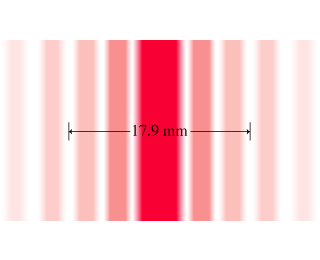
\includegraphics{101966.jpg}}
  \begin{alist}
    \item $45.3\,\mum$
    \item $56.6\,\mum$
    \item $136\,\mum$
    \item $170\,\mum$
    \item $212\,\mum$\correct
  \end{alist}

\item \source{(from Chapter 23+25 homework)} The Balmer series can be
  expressed as $$
    \frac{1}{\lambda}=R\,\left(\frac{1}{2^2}-\frac{1}{n^2} \right) \quad,
  $$ where $\lambda$ is the wavelength of a spectral line, $n$ is any
  integer greater than 2, and $R= 1.097\times 10^7\,\m^{-1}$.  For
  what values of $n$ is $\lambda > 500\,\nm$?\begin{alist}
    \item $n > 3$
    \item $n < 5$
    \item $n < 8$
    \item $n = 7$
    \item none of the above\correct
  \end{alist}

\item \source{(from lecture, 2009-02-02)} If you want to see diffraction
  from an atomic crystal (for example, a copper crystal), what
  wavelength of light should you use?\begin{alist}
    \item $10^{-4}\,\m$
    \item $10^{-6}\,\m$
    \item $10^{-8}\,\m$
    \item $10^{-10}\,\m$\correct
    \item $10^{-12}\,\m$\correct
  \end{alist}

\item \source{(from exercise 23.2)} A $5.0$-$\cm$-thick layer of water
  ($n=1.33$) is sandwiched between a $1.0$-$\cm$-thick sheet of glass
  ($n=1.50$) and a $2.0$-$\cm$-thick sheet of polystyrene plastic
  ($n=1.59$).  How long does it take light incident perpendicular to
  the glass to pass through this $8.0$-$\cm$-thick stack of
  materials?\begin{alist}
    \item $0.19\,\ns$
    \item $0.27\,\ns$
    \item $0.38\,\ns$\correct
    \item much less time than any of those options
    \item much more time than any of those options
  \end{alist}

\item \source{(from lecture, 2009-02-04)} A light ray goes from air
  ($n=1$) to an unknown transparent material.  It is incident on the
  air--material interface at an angle of $30.0\,\deg$ (relative to the
  normal).  It is transmitted into the material at the new angle of
  $18.0\,\deg$.  What is the index of refraction of the
  material?\begin{alist}
    \item 0.62
    \item 0.91
    \item 1.10
    \item 1.62\correct
    \item 1.67
  \end{alist}

\item \source{(from Chapter 23+25 homework)} What is the critical angle
  $\theta_{\mathrm crit}$ for light propagating from a material with
  index of refraction of 1.65 to a material with index of refraction
  of 1.00?  That is, at what angle does refraction start to become
  impossible and total internal reflection kicks in?  Recall that
  angles are measured relative to the normal direction to the
  interface.\begin{alist}
    \item $0.651\,\rad$\correct
    \item $0.651\,\deg$
    \item $0.730\,\rad$
    \item $0.730\,\deg$
    \item $0.920\,\rad$
  \end{alist}

\item \source{(from lecture, 2009-02-09)} If a bug is a distance $D<f$
  away from a thin converging lens of focal length $f$, the image of
  the bug is:\begin{alist}
    \item real and inverted
    \item virtual and inverted
    \item real and not inverted
    \item virtual and not inverted\correct
    \item there is no image in this case
  \end{alist}

\item \source{(from lecture, 2009-02-09)} Consider a simple camera with
  one converging lens of focal length $2.00\,\cm$ with a CCD behind
  it.  If you are focusing on an object a distance $100\,\cm$ away, at
  what distance from the lens should you put the CCD to capture the
  image in focus?\begin{alist}
    \item a lot closer than $2.00\,\cm$
    \item a bit closer than $2.00\,\cm$
    \item at exactly $2.00\,\cm$
    \item a bit farther than $2.00\,\cm$\correct
    \item a lot farther than $2.00\,\cm$
  \end{alist}

\end{enumerate}
\end{document}
